\documentclass[11pt]{article}
\usepackage{geometry}                % See geometry.pdf to learn the layout options. There are lots.
\geometry{letterpaper}                   % ... or a4paper or a5paper or ... 
%\geometry{landscape}                % Activate for for rotated page geometry
%\usepackage[parfill]{parskip}    % Activate to begin paragraphs with an empty line rather than an indent
\usepackage{graphicx}
\usepackage{amssymb}
\usepackage{amsmath}
\usepackage{epstopdf}
\usepackage{hyperref}
\DeclareGraphicsRule{.tif}{png}{.png}{`convert #1 `dirname #1`/`basename #1 .tif`.png}


\graphicspath{
{/Users/Andy/Cruises_Research/Analysis/Andy_Pickering/eq14_patch_gamma/figures/}
}

\title{EQ14 - effect of different fmax in chipod results}
\author{Andy Pickering}
%\date{}                                           % Activate to display a given date or no date



\begin{document}
\maketitle

\tableofcontents
\newpage

%~~~~~~~~~~~~~~~~~~~~~
\section{Overview}

Looking at the effect of using different values for fmax in $\chi$pod processing. 





%~~~~~~~~~~~~~~~~~~~~~~~~~~~~~~~~~~~~~~
\section{Methods}

\begin{itemize}


\end{itemize}


\begin{figure}[htbp]
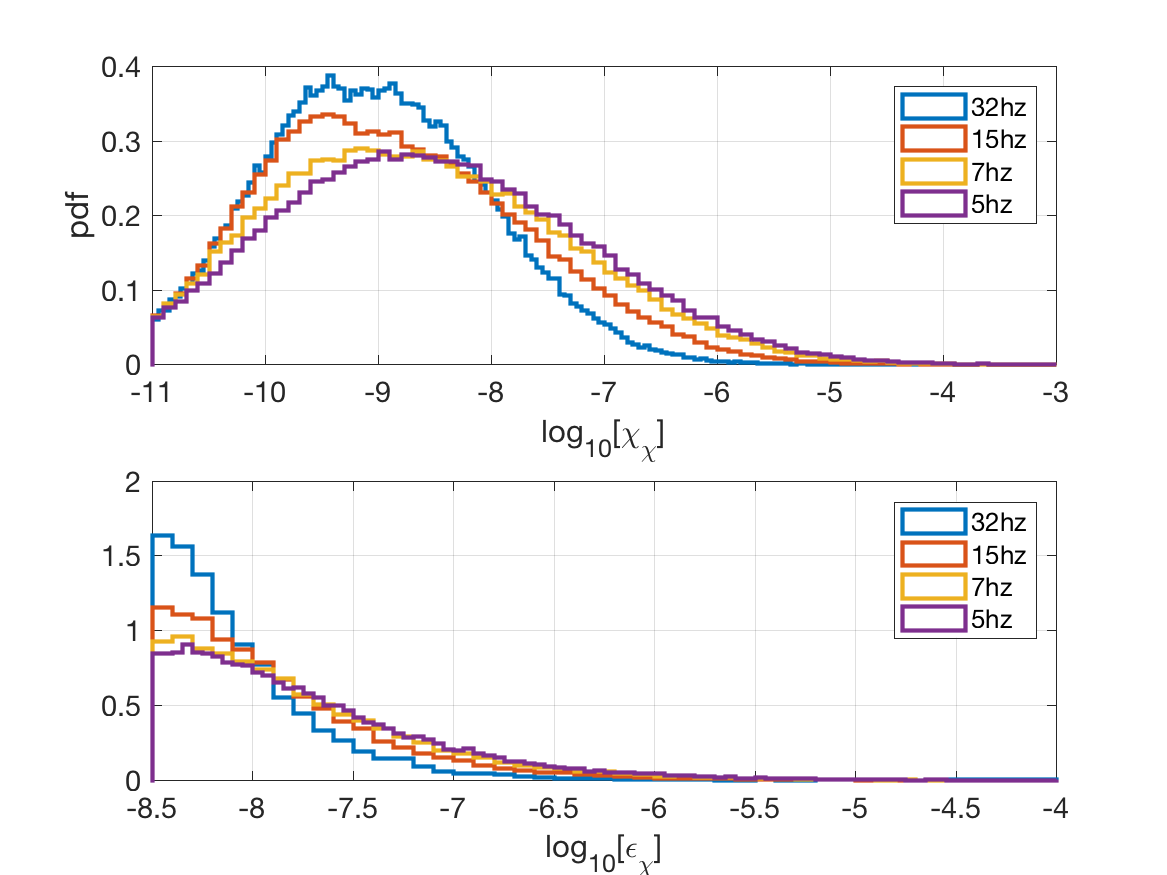
\includegraphics[scale=0.8]{eq14_chi_eps_histograms_diff_fmax.png}
\caption{Histograms of $\chi_{\chi}$ and $\epsilon_{\chi}$ for different values of fmax.}
\label{}
\end{figure}

\begin{figure}[htbp]
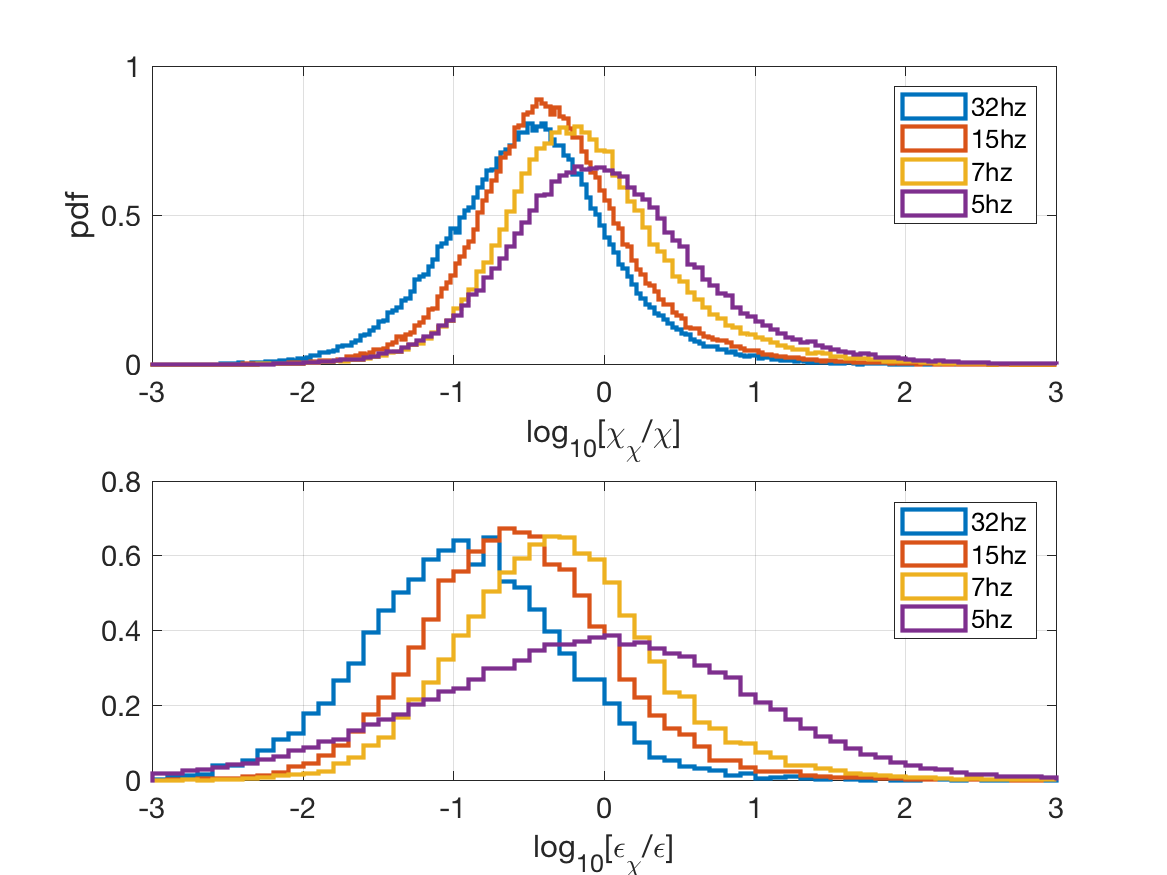
\includegraphics[scale=0.8]{eq14_chi_eps_ratio_histograms_diff_fmax.png}
\caption{Histograms of the ratio of  $\chi_{chi}/\chi$ and $\epsilon_{\chi}\epsilon$ for different values of fmax.}
\label{}
\end{figure}



\begin{figure}[htbp]
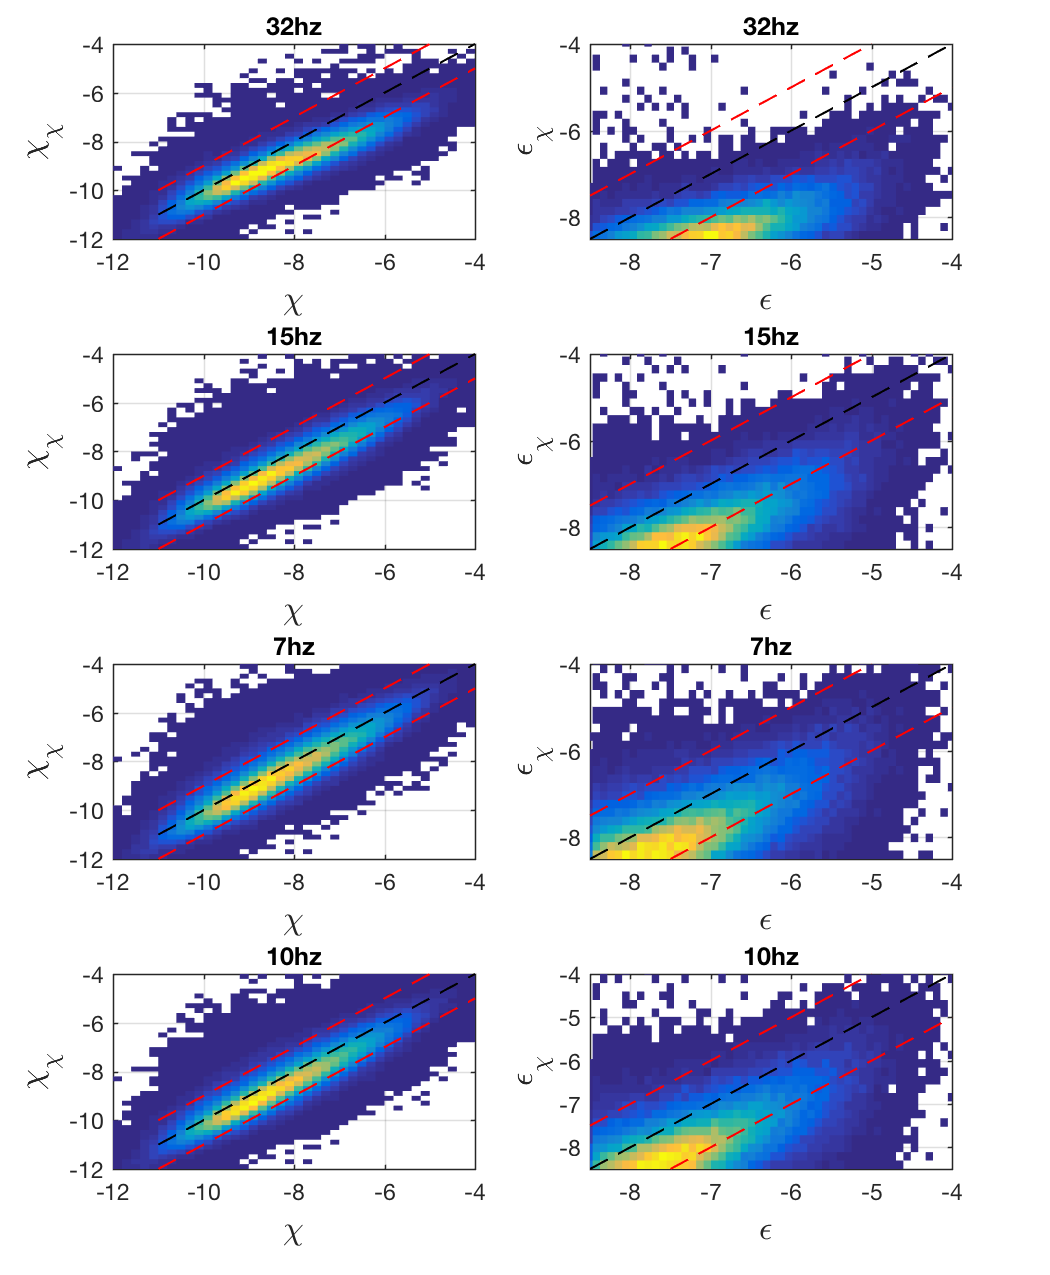
\includegraphics[scale=0.8]{eq14_chi_eps_2Dhistograms_diff_fmax.png}
\caption{2D Histograms of $\chi_{chi}$ vs $\chi$ and $\epsilon_{\chi}$ vs $\epsilon$ for different values of fmax.}
\label{}
\end{figure}





\end{document}  


